%!TEX root = vaisagh_thesis.tex

\chapter{Model Class Structure}


\begin{sidewaysfigure}[!htb]
\centering
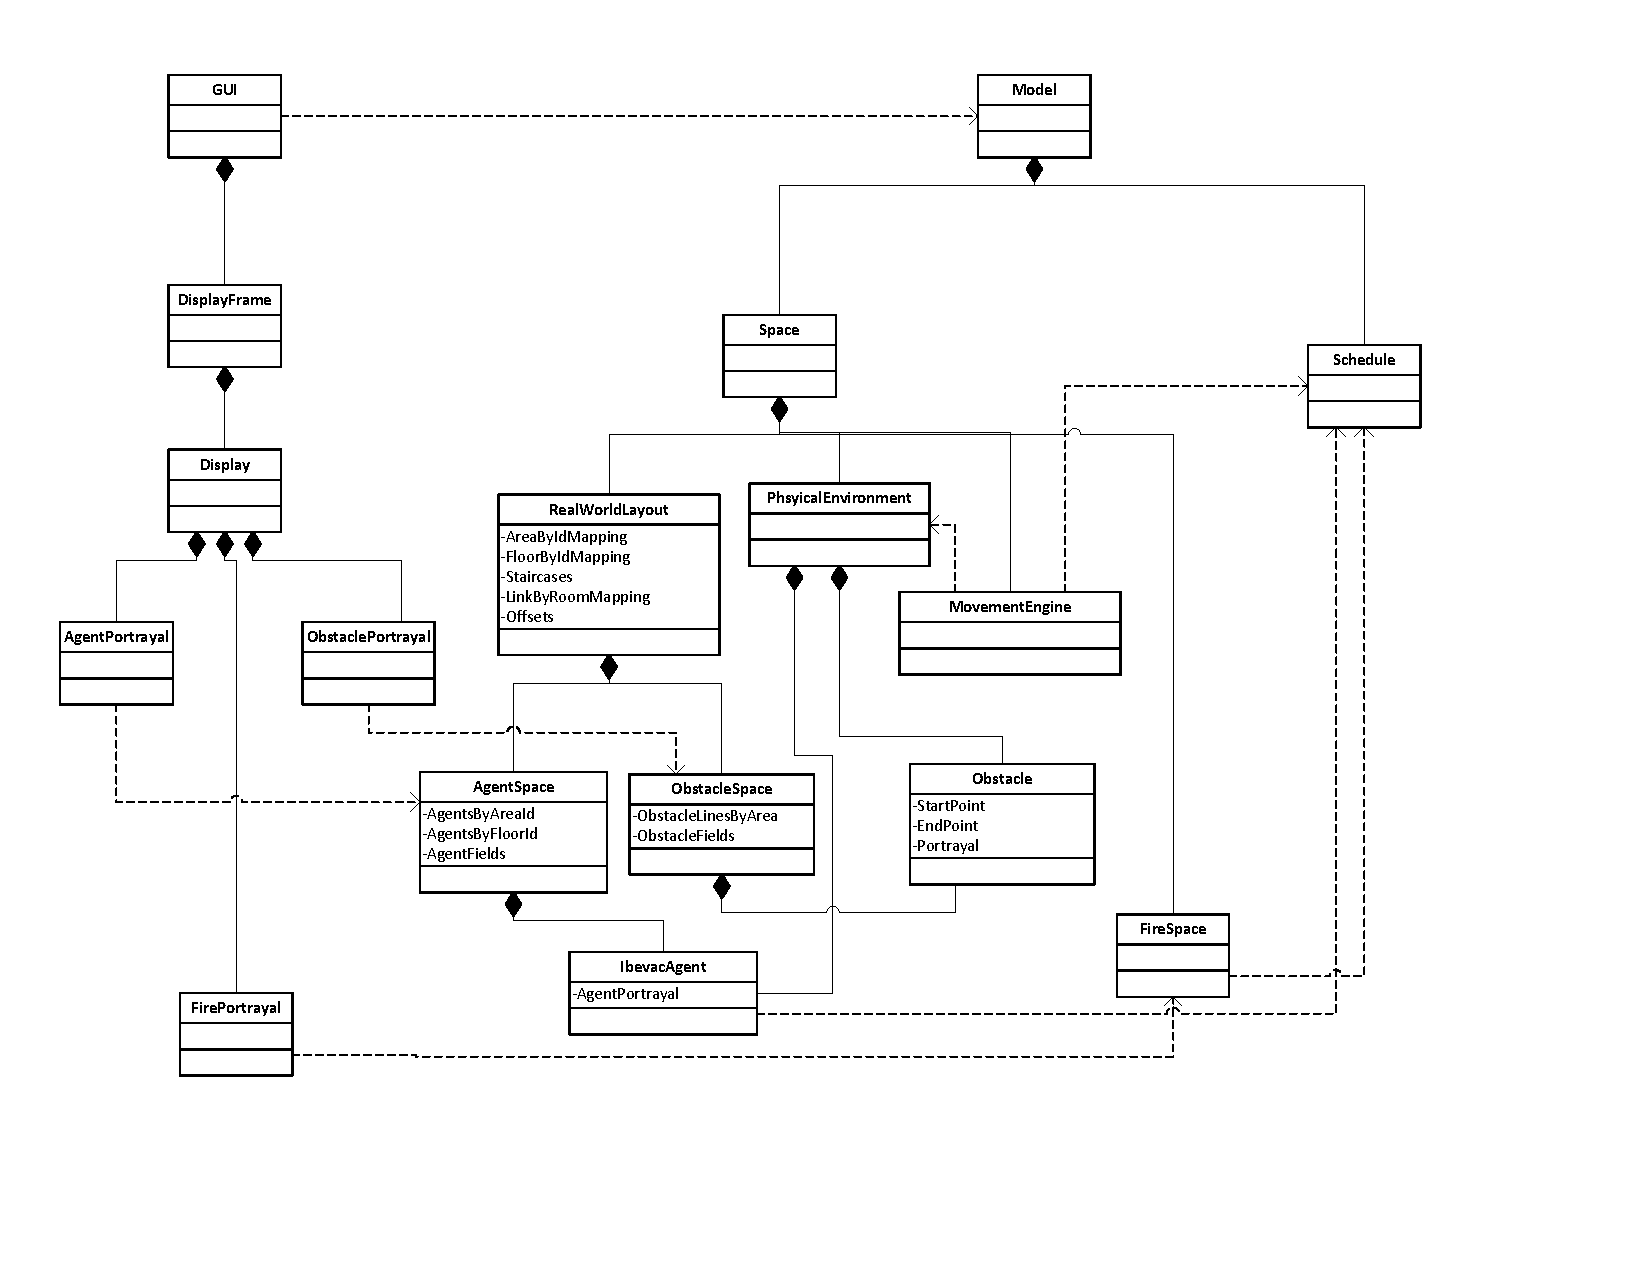
\includegraphics[height=6in, width=11in]{OverallClassStructure}
\caption[Overall Class Structure]{Class Diagram shows the overall class structure of the model}
\label{fig:OverallClassDiagram}
\end{sidewaysfigure}

Figure~\ref{fig:OverallClassDiagram} shows the overall class structure of the model. As can be seen in the diagram, the visualization of the model (IBEVACGui Class) is decoupled from the model itself (IBEVACModel). This allows the modeler to run batches of simulations faster and without interruption. The IBEVACModel class contains the scheduler that runs the simulation and it also holds an instance of the Simulation Space. To effectively consider and model each different part of the model, the Space class delegates most of its functions to the classes within it. Of this, the fireSpace uses the scheduler to simulate the spreading of the fire and stores in the form of a field that can be used by the Portrayal Instance in the visualization class to render the fire. The Physical Environment and the level 0 motion classes are used to ensure the consistency of the environment. The remaining class is the space in which the agents and obstacles are stored. This space also stores information on the relationships between areas, floors and links. Again, delegation is used to maximize modularity and minimize the dependencies between the different classes.

\begin{sidewaysfigure}[!htb]
\centering
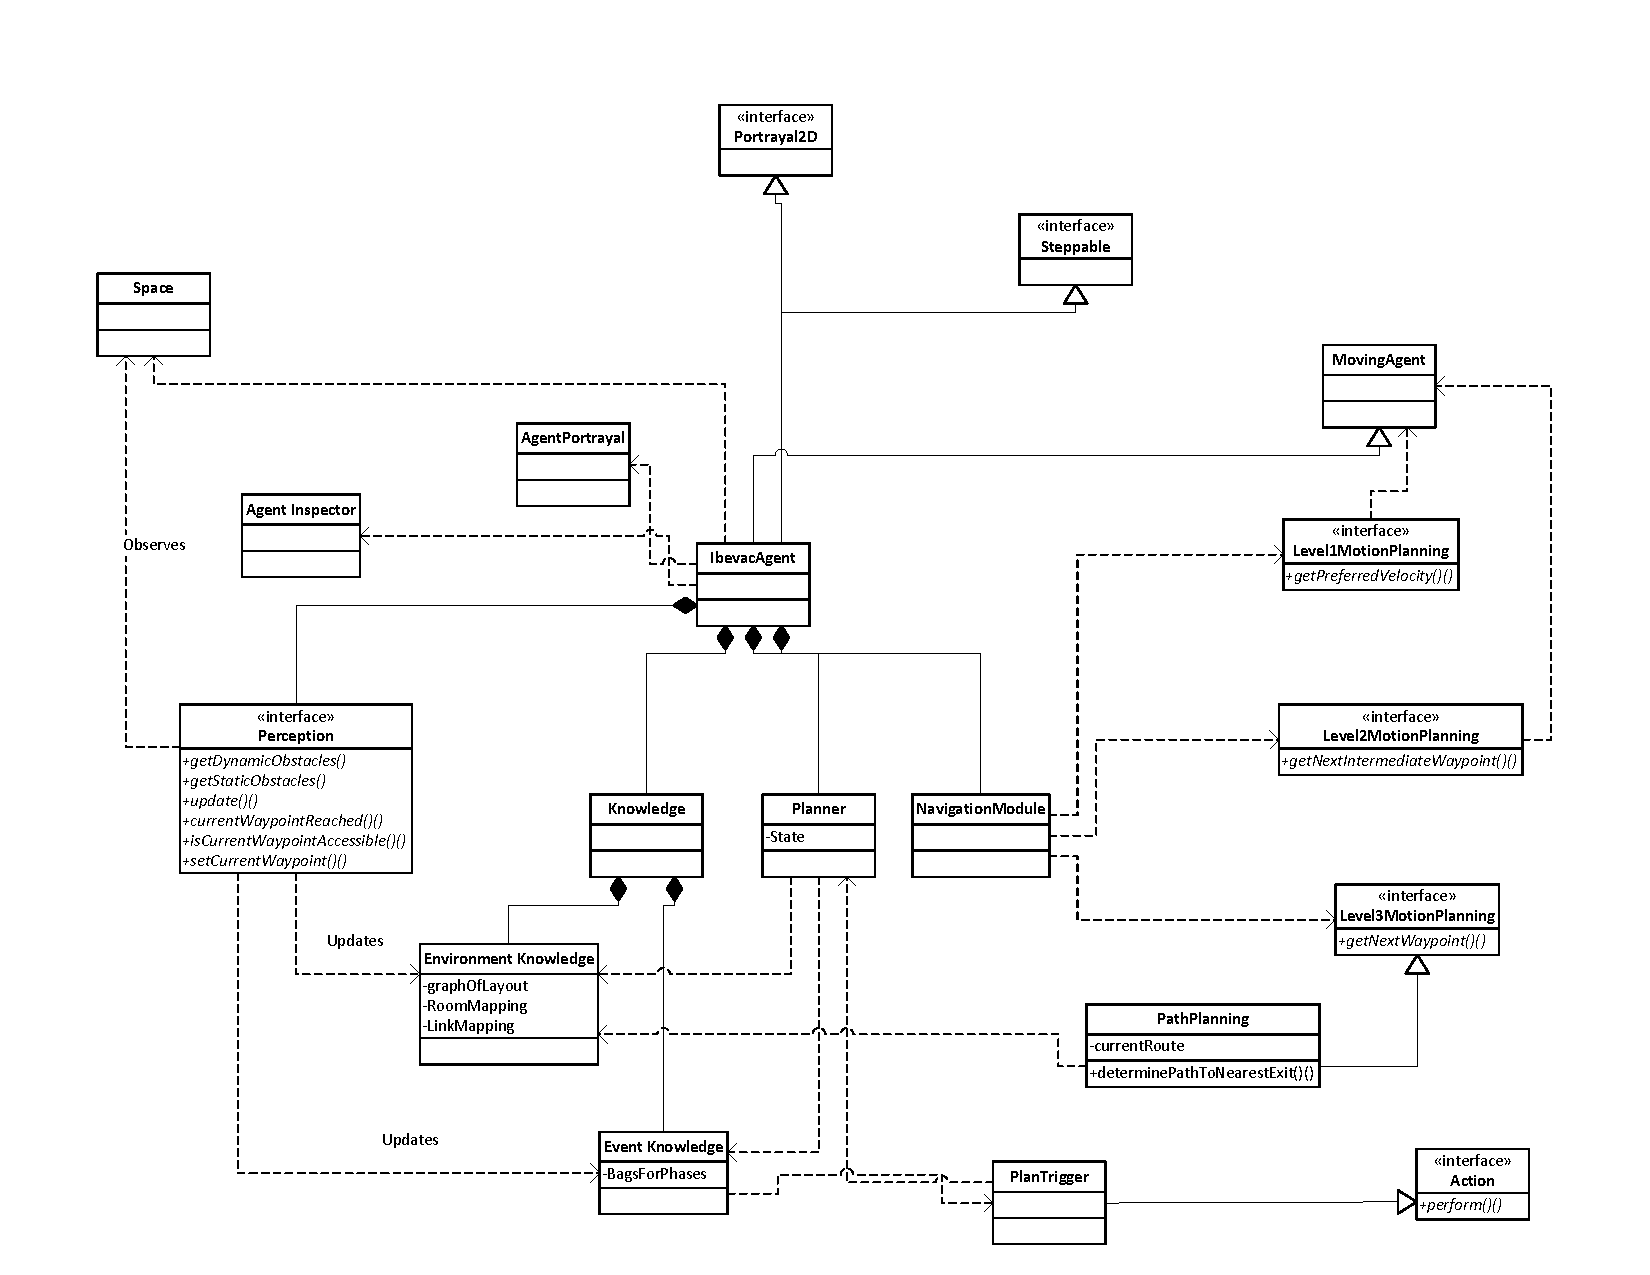
\includegraphics[height=6in,width=11in]{AgentClassStructure}
\caption[Agent Class Structure]{This Class Diagram shows the agent class in detail}
\label{fig:AgentClassDiagram}
\end{sidewaysfigure}

The Agent class in the Fig.~\ref{fig:OverallClassDiagram} is shown in more detail in Fig.~\ref{fig:AgentClassDiagram}. This is the entity that implements the behavior of the agent. Classes like the Agent Portrayal and Agent Inspector are responsible for displaying the agent and displaying and editing values of a particular agent. The IbevacAgent delegates these tasks to these classes. The IBEVAC architecture explained in Chapter~\ref{chapter:IBEVAC} is modeled almost exactly as suggested by the architecture and the class diagram illustrates this clearly.

The agent's perception is modeled as an interface so that the perception system can easily be extended and improved at a later date without affecting the rest of the model. During each step of the model, the agent's perception is first updated. This perception updates the environment and event knowledge base of the agent. Changes in the environment and event knowledge can trigger a plan change in the planner. Depending on the current state and activity being completed by the agent, the planner passes a goal point to the navigation module which generates the velocity and movement of the agent in each time step.

One of the key novelties of the IBEVAC model is in the way that cues are modeled. Different kinds of cues are generated by the environment and the agents. Each cue implements the Cue interface. Each agent can sense these Cue type objects from the environment and react to them.
